\documentclass[12pt]{article}
\usepackage{polski}
\usepackage[utf8]{inputenc}
\usepackage[margin=1in]{geometry}
\usepackage[english,polish]{babel}
\usepackage{graphicx}
\usepackage{indentfirst}
\usepackage{graphicx} 
\usepackage{float}
\usepackage{textcomp}
\usepackage{caption}
\usepackage{listings}
\usepackage{color}
\usepackage{hyperref}

\lstset{language=Python,
                keywordstyle=\color{blue},
                stringstyle=\color{red},
                morecomment=[l][\color{magenta}]{\#},
                showspaces=false,
                showstringspaces=false,
                frame=single
}

\begin{document}
\thispagestyle{empty}

\begin{flushright}\today\end{flushright}

\noindent
Mateusz Burniak 218321 \\
Artur Malarz 218355 \\
Szymon Janora 218361 \\

\vspace{1em}

\noindent
grupa: środa, $7^{30}$-$9^{00}$

\vfill

\begin{center}
  \begin{Large}
DOKUMENTACJA PROJEKTU
  \end{Large}

\vspace{2cm}
 

  \begin{Huge}
BOJAMO 

  \end{Huge}
  
 \vspace{1cm}
  
  \begin{Large}

Project Management Software

  \end{Large}
\end{center}

\vspace{3cm}
 
\noindent
  \begin{Large}
    Prowadzący: \\
      \vspace{.5cm}
\indent
Mgr inż. Agnieszka Kaczmarek
  \end{Large}


  \vspace{1cm}
  
\noindent
  \begin{Large}
    Rok akademicki: \\
      \vspace{.5cm}
\indent
2016/2017
  \end{Large}
  

\vfill

\newpage

\tableofcontents

\newpage


\section{Założenia projektowe}

    Celem projektu jest zaimplementowanie zgodnego z metodyką SCRUM oprogramowania do zarządzania projektami, w postaci aplikacji internetowej oraz projekt i implementacja bazy danych, na której omawiana aplikacja będzie operować.

\subsection{Dane techniczne}

\begin{itemize}
\item
Do implementacji BackEndu zostanie wykorzystany język programowania Python 3.51 oraz dostępny dla tego języka framework Django 1.10.
\item
Do zarządzania implementowaną bazą danych zostanie wykorzystany system PostgreSQL i SQLite (początkowa faza projektu).
\item
Do implementacji FrontEndu zostanie wykorzystany framework Twitter BootStrap 3.
\item
W celu przeprowadzenia wirtualizacji środowiska, w którym pracować będzie system bazodanowy zostanie wykorzystane oprogramowanie Docker.
\item
W celu komunikacji i zarządzania danymi zawartymi w bazie danych zostanie wykorzystane mapowanie obiektowo-relacyjne, dzięki czemu aplikacja będzie kompatybilna z wieloma systemami bazodanowymi.

\end{itemize}

\subsection{Funkcjonalności}
\begin{itemize}
\item
Aplikacja musi spełniać rolę menadżera projektów zgodnego z metodyką SCRUM, co za tym idzie musi dostarczać odpowiednie funkcjonalności i mechanizmy pozwalające na pracę zgodną z założeniami wybranej metodyki. 
\item
Zgodnie z metodyką użytkownik będzie mógł wybierać odpowiadające mu zadania lub tworzyć nowe w obrębie aktywnego sprintu będącego elementem prac wykonywanych nad projektem w okresie czasu. Powinno być możliwe rozróżnienie zadań pod względem kategorii oraz wagi. 
\item
Oprogramowanie musi pozwalać na śledzenie postępów prac wykonanych w projekcie, w związku z tym użytkownicy będą mieć możliwość logowania czasu spędzonego nad wykonywanym zadaniem.
\item
Oprogramowanie musi zawierać podstawowe zabezpieczenia w postaci walidacji użytkownika oraz jego dostępu do danych zasobów, aplikacja ma dostarczać podstawowe funkcje takie jak logowanie/rejestracja. Hasła muszą być odpowiednio zabezpieczone przed wyciekiem, w związku z tym zostanie wykorzystane szyfrowanie SHA2 z solą. 


\end{itemize}


\subsection{Schemat bazy danych}
\newgeometry{top=0cm}
\begin{figure}[htp]
\centering
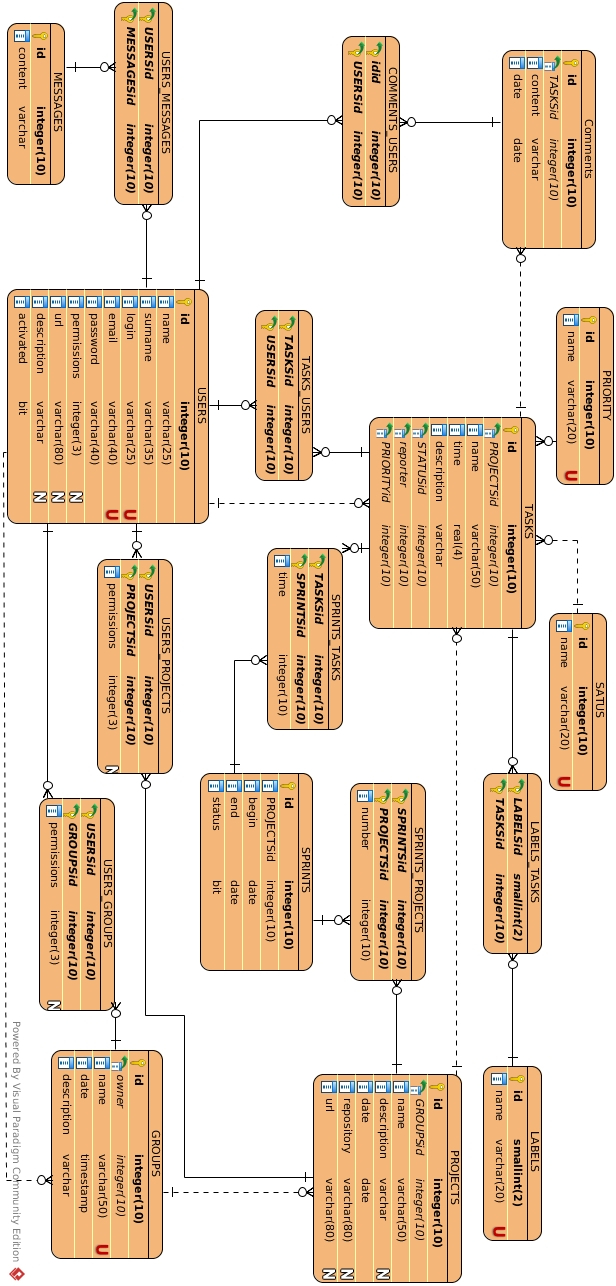
\includegraphics[scale=0.61]{img/db_schema.jpg}
\caption{}
\label{}
\end{figure}
\restoregeometry

\section{Opis implementacji}
    Realizowany przez nas projekt został zaimplementowany zgodnie ze wspieranym przez framework Django wzorcem MVC (Model View Controller), a ponadto aplikacje podzielono na pomniejsze serwisy według modeli bazy danych na których one operowały.
    

\subsection{Struktura projektu}

\begin{figure}[htp]
\centering
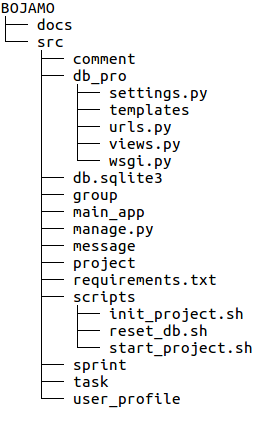
\includegraphics[scale=0.7]{img/tree.png}
\caption{Schemat projektu}
\label{}
\end{figure}

Aplikacja db-pro jest głównym serwisem projektu, odpowiada ona za podstawowy routing i działa jak główny kontroler wywołujący pozostałe serwisy.  

Struktura folderu zawierającego serwis odpowiadający za operowanie na danych modelach, została przedstawiona na podstawie aplikacji group. Jak widać aplikacja group jak również pozostałe składa się z kilku plików oraz folderów migrations i templates. Folder migrations zawiera pliki wspierające ORM, wygenerowane przez Django i  odpowiadające za migrację danych. Folder templates zawiera szablony stron wykorzystujące technologię HTML oraz Jinja, szablony odpowiadają za prezentację danych użytkownikowi. Jak można zauważyć w folderze aplikacji brakuje pliku controler, którym cechuje się wzorzec MVC, brak kontrolera jest cechą frameworka Django, operacje obsługiwane przez kontroler zostały połączone z widokiem, dlatego dostępne mamy jedynie pliku models.py oraz views.py. 

\begin{itemize}
\item
models.py - odpowiada za utworzenie encji w bazie danych, odpowiadającej zapisanemy w języku Python obiektowi. 
\item
urls.py - zawiera zapis routingu dla danego serwisu
\item
views.py - łaczy w sobie funkcję widoku oraz kontrolera, służy do wyświelania odpowiednich szablonów, operowaniu na danych oraz przekierowywaniu operacji do innych aplikacji.
\item
admin.py - pozwala zmodyfikować stronę administratora udostępnianą przez framework Django, wprowadzając widoki danej aplikacji i pozwalająć na operowanie bazą danych w obrębie modeli dostępnych dla aplikacji.  
\item
forms.py - przechowuje kod odpowiedzialny za utworzenie formularzy dla danego modelu oraz reguły walidacji jego poprawności.

\end{itemize}

W strukturze projektu można zauważyć plik bazy danych SQLite 3, jest to podstawowa baza danych, domyślnie tworzona przez framework. Omawiany system zarządzania bazą danych był wykorzystywany przez nas w początkowej fazie projektu, podczas dalszych prac i utworzeniu wszystkich potrzebnych nam modeli, zamieniliśmy omawiany system na PostgreSQL uruchamiany w wirtualnym kontenerze aplikacji Docker. Ze względu na zmianę systemu bazy danych został wprowadzony zestaw skryptów powłoki Bash, które dostępne są w folderze scripts  i umożliwiają one inicjacje danymi, uruchomienie, czy restart kontenera Docker z PostgreSQL. Obie wykorzystywane bazy danych zostały wypełnione wygenerowanymi przez nas danymi testowymi. 

\subsection{Przykłady implementacji}

\subsubsection{Implementacja routingu}

\begin{lstlisting}[caption={groups/urls.py}]
from django.conf.urls import url

from project.views import ProjectCreateView
from .views import GroupCreateView, group_detail

urlpatterns = [
    url(r'^create/$', GroupCreateView.as_view(),
        name='group_create_view'),
    url(r'^(?P<name>\w+)/$', group_detail,
        name='group_detail'),
    url(r'^(?P<group>\w+)/add/$', ProjectCreateView.as_view(),
        name='project_create_view'),
]
\end{lstlisting}

    Aplikacja pobiera każdy z adresów należących do jej domeny, w przypadku fazy rozwojowej jest to adres domeny 127.0.0.1:8000. Odpytanie aplikacji adresem z parametrami powoduje próbę dopasowania adresu do zadanych wzorców w formie wyrażeń regularnych, po dopasowaniu adresu zostaje wywołany przypisany do niego widok lub w przypadku głównego routingu, parametry z adresu zostają przekazane do przypisanej aplikacji. 
    
Przykładowo, dopasowanie adresu 127.0.0.1:8000/group\_name/add spowoduje wywołanie widoku ProjectCreateView, który umożliwi stworzenie nowego projektu przypisanego do grupy o nazwie group\_name.


\subsubsection{Implementacja modelu}

\begin{lstlisting}[caption={groups/models.py}]
from django.contrib.auth.models import User
from django.db import models


class Group(models.Model):
    owner = models.ForeignKey(
        User
    )
    name = models.CharField(
        max_length=50
    )
    date = models.DateField(
        auto_now=True
    )
    description = models.TextField(
        blank=True,
        null=True
    )

    def __str__(self):
        return self.name


class UserGroup(models.Model):
    user = models.ForeignKey(User)
    group = models.ForeignKey(Group)
    permissions = models.PositiveSmallIntegerField(default=1)

    def __str__(self):
        return '({}, {})'.format(self.user.username, self.group)

    class Meta:
        unique_together = ['user', 'group']
\end{lstlisting}

    Powyższy widok przedstawia implementację modeli obiektów Group oraz UserGroup. 
    
System ORM wspierany przez Django, pozwala na proste tworzenie obiektów bazy danych, których implementacja przechowywana jest w kodzie języka Python. Ponadto system ten pozwala na przeładowanie metod odziedziczonych po klasie bazowej Model, co można zauważyć przykładowo po przeładowanej metodzie \_\_str\_\_, zwracającej tekstową reprezentację obiektu. Poza tym framework Django umożliwia proste tworzenie relacji pomiędzy modelami/encjami, co jest widoczne w implementacji modelu UserGroup, stanowiącego relację pomiędzy modelem User i modelem Group. 


\subsubsection{Implementacja formularza}

\begin{lstlisting}[caption={groups/forms.py}]
from django import forms
from .models import Group


class GroupForm(forms.ModelForm):
    class Meta:
        model = Group
        fields = {'name', 'description'}
        widgets = {
            'name': forms.TextInput(
                attrs={
                    'class': 'form-control',
                }
            ),
            'description': forms.Textarea(
                attrs={
                    'class': 'form-control'
                }
            )
        }
\end{lstlisting}

    Framework Django pozwala na prostą obiektową implementację formularzy, co przedstawia powyższy widok, na którym widoczna jest implementacja formularza służącego do utworzenia obiektu modelu Group. Django pozwala ponadto na przeładowanie metod odziedziczonych po klasie bazowej ModelForm, co pozwoli chociażby na utworzenie metody służącej do walidacji poprawności wypełnionego formularza.  

\subsubsection{Implementacja widoku administratora}

\begin{lstlisting}[caption={groups/admin.py}]
from django.contrib import admin

from .models import Group, UserGroup

admin.site.register(Group)
admin.site.register(UserGroup)
\end{lstlisting}

Poprzez wywołanie metody register(model\_type) dostępnej dla podstrony administratora, z podanym w parametrze modelem pozwala na dodanie funkcjonalności w widoku administratora, pozwalających na operowanie bazą danych w obrębie zadanego modelu.


\subsubsection{Implementacja widoków aplikacji}

\begin{lstlisting}[caption={groups/views.py}]
from django.contrib.auth.decorators import login_required
from django.contrib.auth.models import User
from django.http import HttpResponseRedirect
from django.shortcuts import get_object_or_404, render
from django.urls import reverse_lazy
from django.utils.decorators import method_decorator
from django.views.generic import CreateView, ListView

from project.models import Project
from .forms import GroupForm
from .models import Group, UserGroup


class GroupCreateView(CreateView):
    model = Group
    form_class = GroupForm
    template_name = 'group/create_view.html'
    success_url = 'user_profile/loggedin.html'

    def get_context_data(self, **kwargs):
        context = super().get_context_data(**kwargs)
        return context

    def form_valid(self, form):
        group = Group.objects.create(owner=self.request.user,
            name=form['name'].value(),
            description=form['description'].value())
        UserGroup.objects.create(user=self.request.user, group=group)
        return HttpResponseRedirect(reverse_lazy('dashboard'))

    @method_decorator(login_required)
    def dispatch(self, *args, **kwargs):
        return super(GroupCreateView, self).dispatch(*args, **kwargs)


class GroupListView(ListView):
    model = Group


@login_required
def group_detail(request, name):
    group = get_object_or_404(Group, name=name)
    owner = User.objects.get(id=group.owner_id)
    members = [i.user for i in UserGroup.objects.filter(group=group)]
    projects = Project.objects.filter(group=group)
    context = {'group': group, 'owner': owner, 'members': members,
        'projects': projects}
    return render(request, 'group/group_detail.html', context)
\end{lstlisting}

    Widoki zostały zaimplementowane na dwa sposoby, podstawowej metody pobierającej obiekt request oraz w sposób obiektowy przy wykorzystaniu widoków generycznych. Wszystkie widoki zostały zabezpieczone fixturą login\_required, która uniemożliwia wywołanie danego widoku użytkownikowi, który nie przeszedł przez proces uwierzytelniania podczas logowania.  


\subsubsection{Implementacja bazy danych}

\begin{lstlisting}[caption={scripts/reset\_db.sh},language=bash]
#!/usr/bin/env bash

docker rm -f bojamo-postgres
docker run \
    --name bojamo-postgres \
    -e POSTGRES_PASSWORD=mysecretpassword \
    -e POSTGRES_USER=user \
    -e POSTGRES_DB=bojamo_db \
    -p 54321:5432 \
    -d postgres:9.5

sleep 10
python3 manage.py makemigrations
python3 manage.py migrate
./apply_mock.py
\end{lstlisting}

Jak widać na powyższym listingu najpierw usuwany jest poptrzedni obraz dockerowy, następnie tworzony jest nowy i aplikowanę są fixtury.


\section{Funkcjonalność projektu}
Niezalogowany użytkownik może się jedynie zalogować lub zarejestrować. Kiedy użytkownik jest już zalogowany, może dodawać nowe projekty, tworzyć grupy projektowe. Do grupy można dodawać nowe sprinty. Do sprintów można przypisywać taski.

\subsection{Screeny działającej aplikacji}

\begin{figure}[htp]
\centering
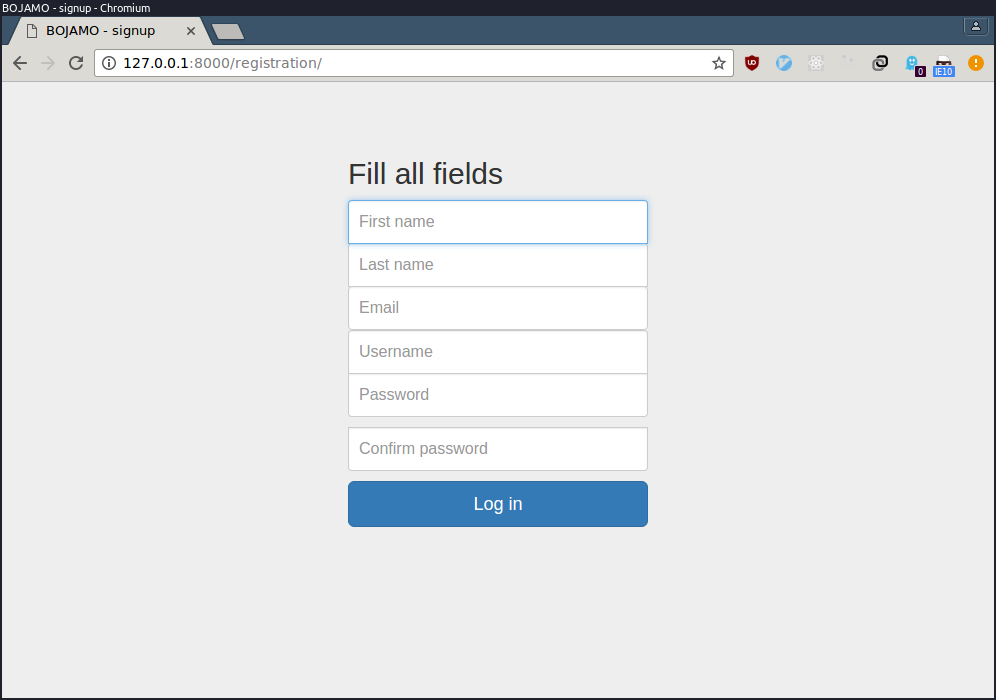
\includegraphics[scale=.5]{img/register.png}
\caption{Rejestracja użytkownika}
\label{}
\end{figure}

\begin{figure}[htp]
\centering
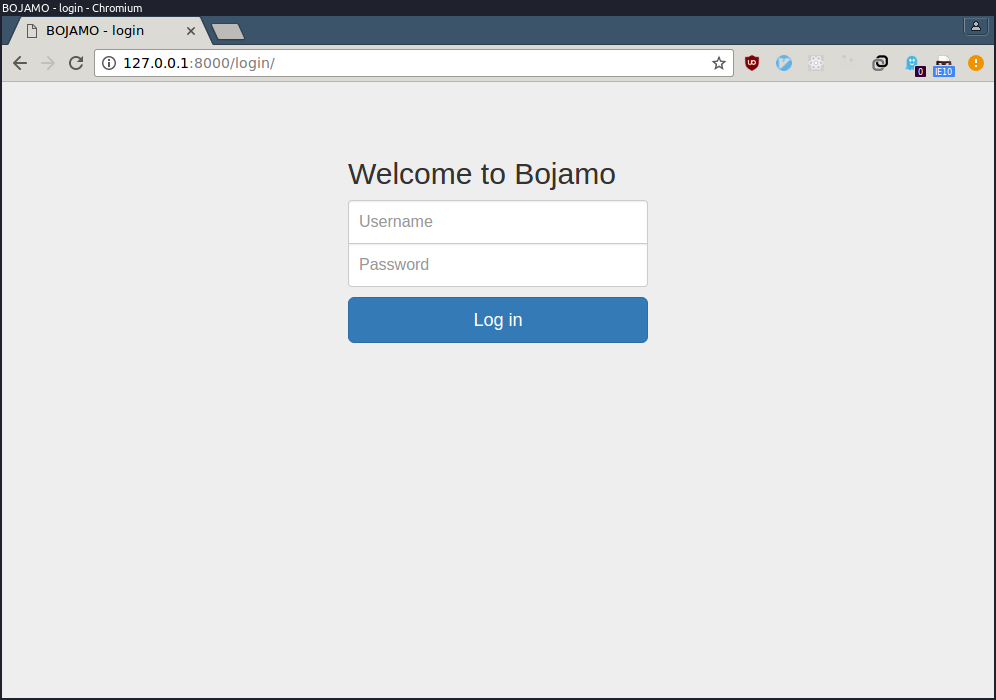
\includegraphics[scale=.5]{img/login.png}
\caption{Logowanie użytkownika}
\label{}
\end{figure}

\begin{figure}[htp]
\centering
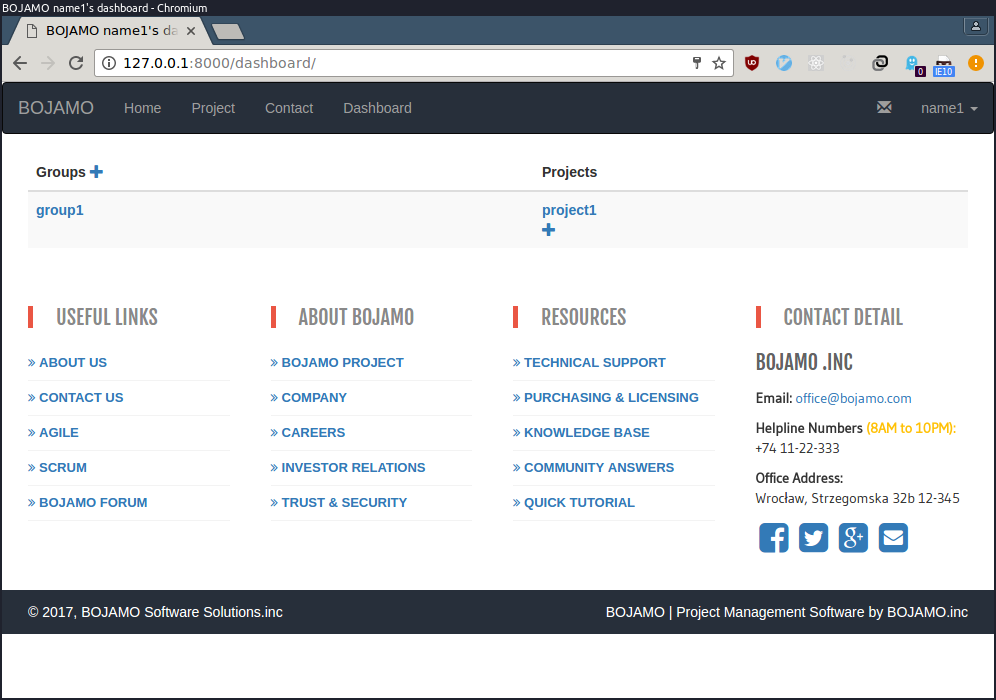
\includegraphics[scale=.5]{img/dashboard.png}
\caption{Widok po zalogowaniu}
\label{}
\end{figure}

\begin{figure}[htp]
\centering
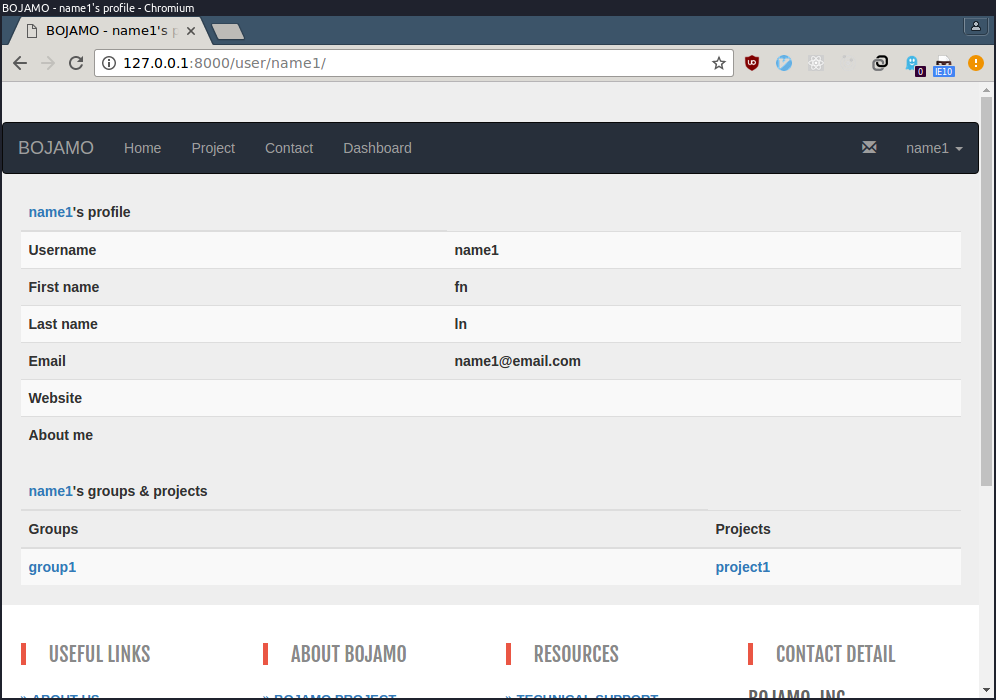
\includegraphics[scale=.5]{img/user.png}
\caption{Widok użytkownika}
\label{}
\end{figure}

\begin{figure}[htp]
\centering
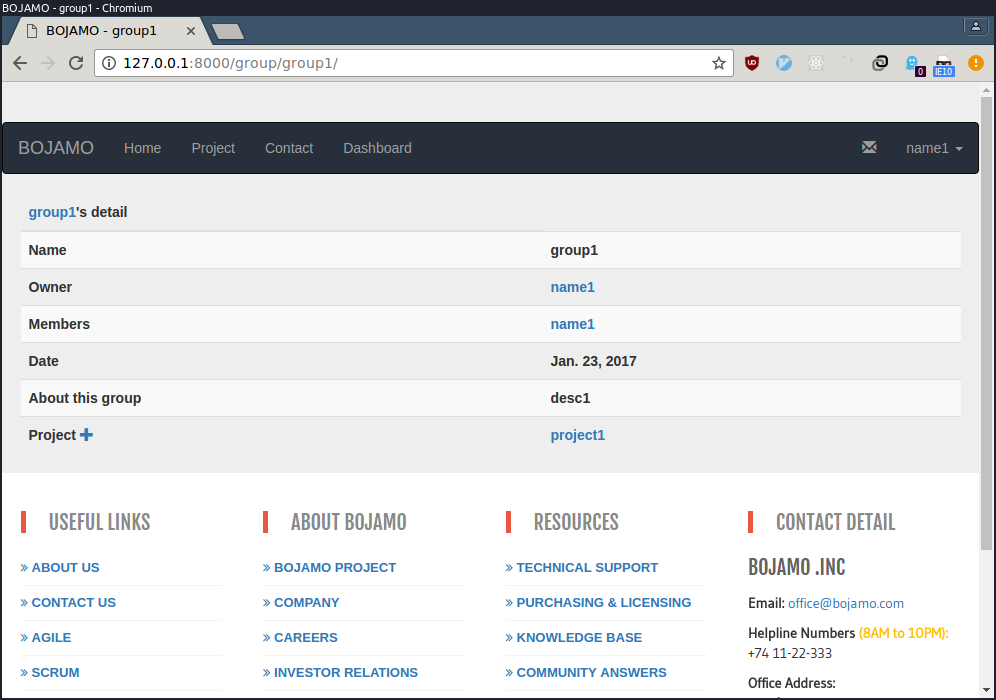
\includegraphics[scale=.5]{img/group.png}
\caption{Widok grupy}
\label{}
\end{figure}

\begin{figure}[htp]
\centering
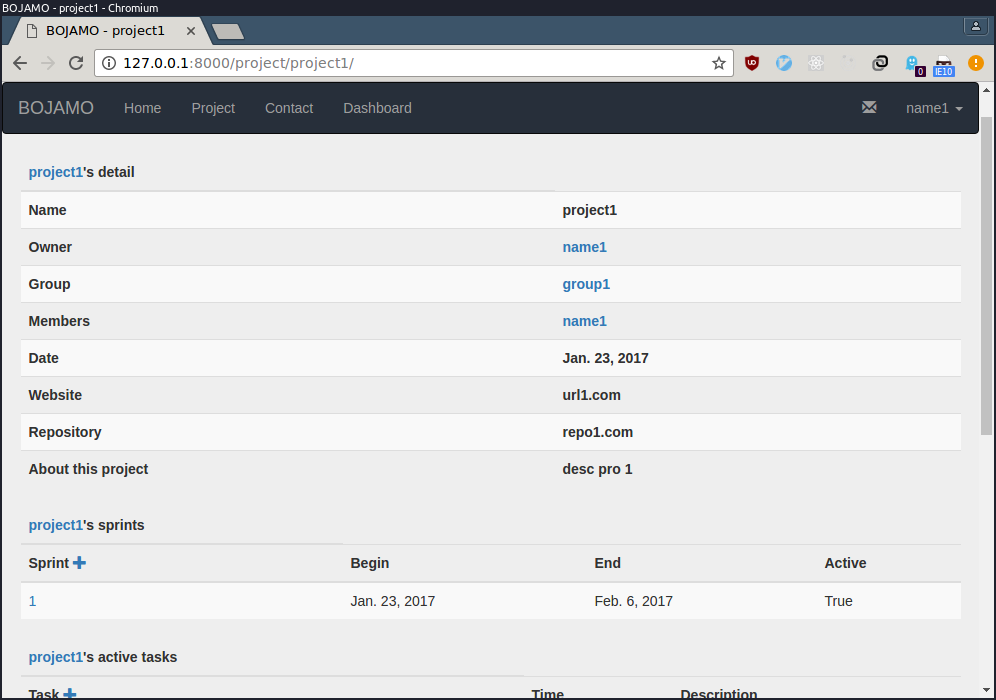
\includegraphics[scale=.5]{img/project.png}
\caption{Widok projektu}
\label{}
\end{figure}

\begin{figure}[htp]
\centering
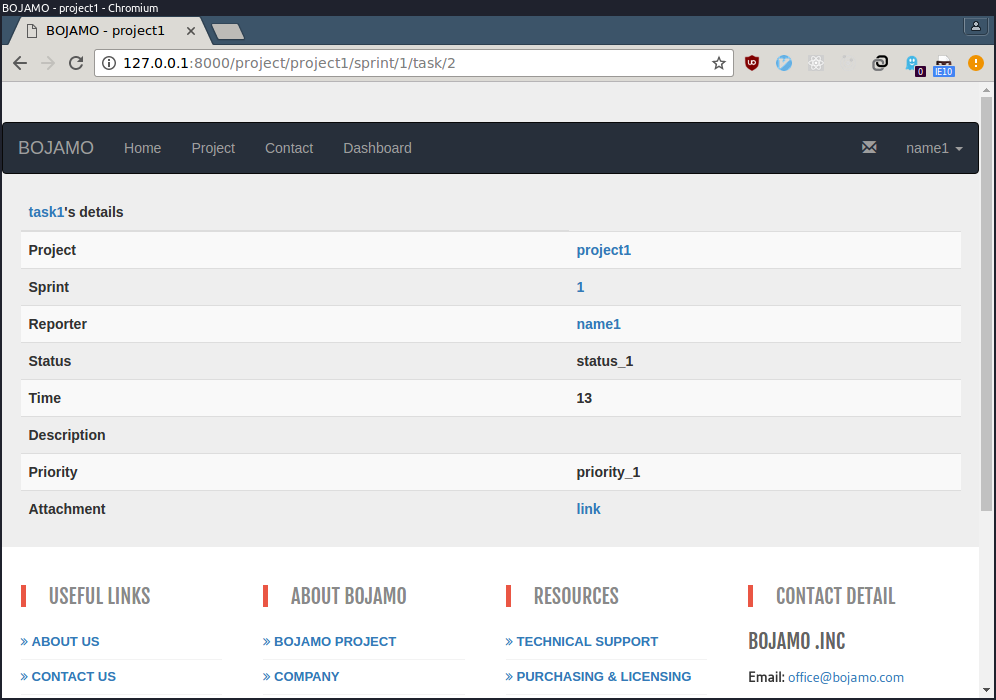
\includegraphics[scale=.5]{img/task.png}
\caption{Widok zadania}
\label{}
\end{figure}

\newpage

\section{Podsumowanie}

Mając gotowe założenia stworzyliśmy kompletny projekt bazy danych oraz aplikacji. W fazie projektowania bazy danych poznaliśmy od podstaw etapy powstawania projektu bazy danych począwszy od diagramu związków encji, aż do powstania modelu fizycznego bazy danych. Podczas projektowania aplikacji poznaliśmy dokładniej Pythona i zasady działania frameworku Django, co pozwoliło nam szybciej stworzyć aplikację.

Jakość kodu jest na wysokim poziomie, zatem możliwy jest dalszy rozwój aplikacji. Korzystamy z najnowszych, obecnie dostępnych, technologii, które zyskują coraz
większą popularność.

Mapowanie obiektowo-relacyjne jest to mechanizm znacznie ułatwiającym pracę z bazą
danych. Dzięki niemu możemy komunikować się z bazą danych używając języka obiektowego zamiast wysyłania zapytań SQL. Ponadto nasza baza danych jest zwirtualizowana przy pomocy Dockera, co zapewnia większą przenośność i skalowalność.


\end{document}